\section{Ежедневное закрытие смены с вводом контрольных сумм}
%\marginnote{\Date{Чт.}{12}{Июл.}{2018}}[-40pt]
	\begin{warning}
		\textbf{Внимание!!!! Перед закрытием смены убедитесь в наличии достаточного количества бумаги в фискальном регистраторе. \\
		В случае возникновения любой ошибки или нестандартной ситуации при работе на кассе, необходимо нажать клавишу <<Скрин>> на клавиатуре.}
	\end{warning}

	

\begin{itemize}
	\item Жмём <<Закрытие смены>>
	
	
	\begin{figure}[H]
		
\includegraphics[width=0.4\textwidth]{1.png}
		\caption{<<Закрытие смены>>}
		\label{ris:1.png}
	\end{figure}
	
	\item Выйдет форма с вопросом. Отвечаем <<Да>>
	\item Еще раз нажимаем <<Закрытие смены>>
	\begin{figure}[H]
		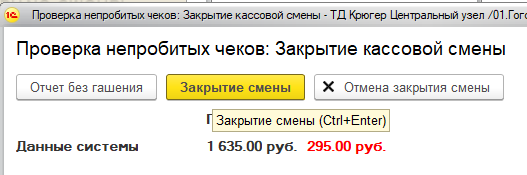
\includegraphics[width=0.6\textwidth]{2.png}
		\caption{<<Закрытие смены далее>>}
		\label{ris:2.png}
	\end{figure}
 	\item Заполняем суммы продаж и возвратов, в форме ввода сумм (Рис.~\ref{ris:3.jpg}) вводя цифры с X-отчета который распечатался на фискальном регистраторе и контрольной ленты эквайринга:
	\begin{figure}[H]
 		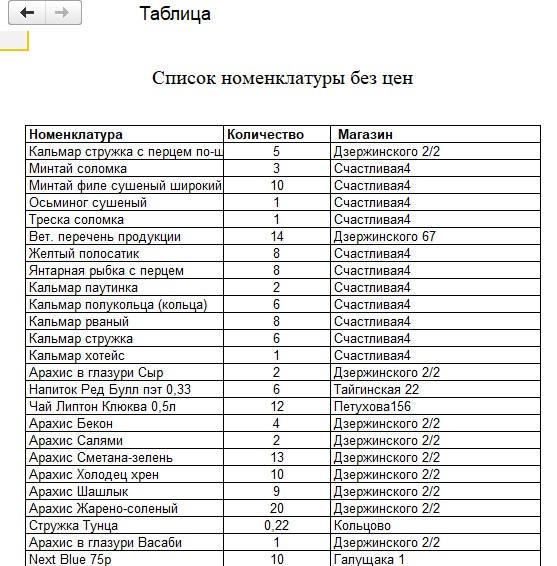
\includegraphics[width=0.6\textwidth]{3.jpg}
 		\caption{<<Ввод сумм>>}
 		\label{ris:3.jpg}
 	\end{figure}
	\par

	
	\begin{figure}[H]
		  \begin{floatrow}
			   \ffigbox{\caption{X-отчет}}%
			   {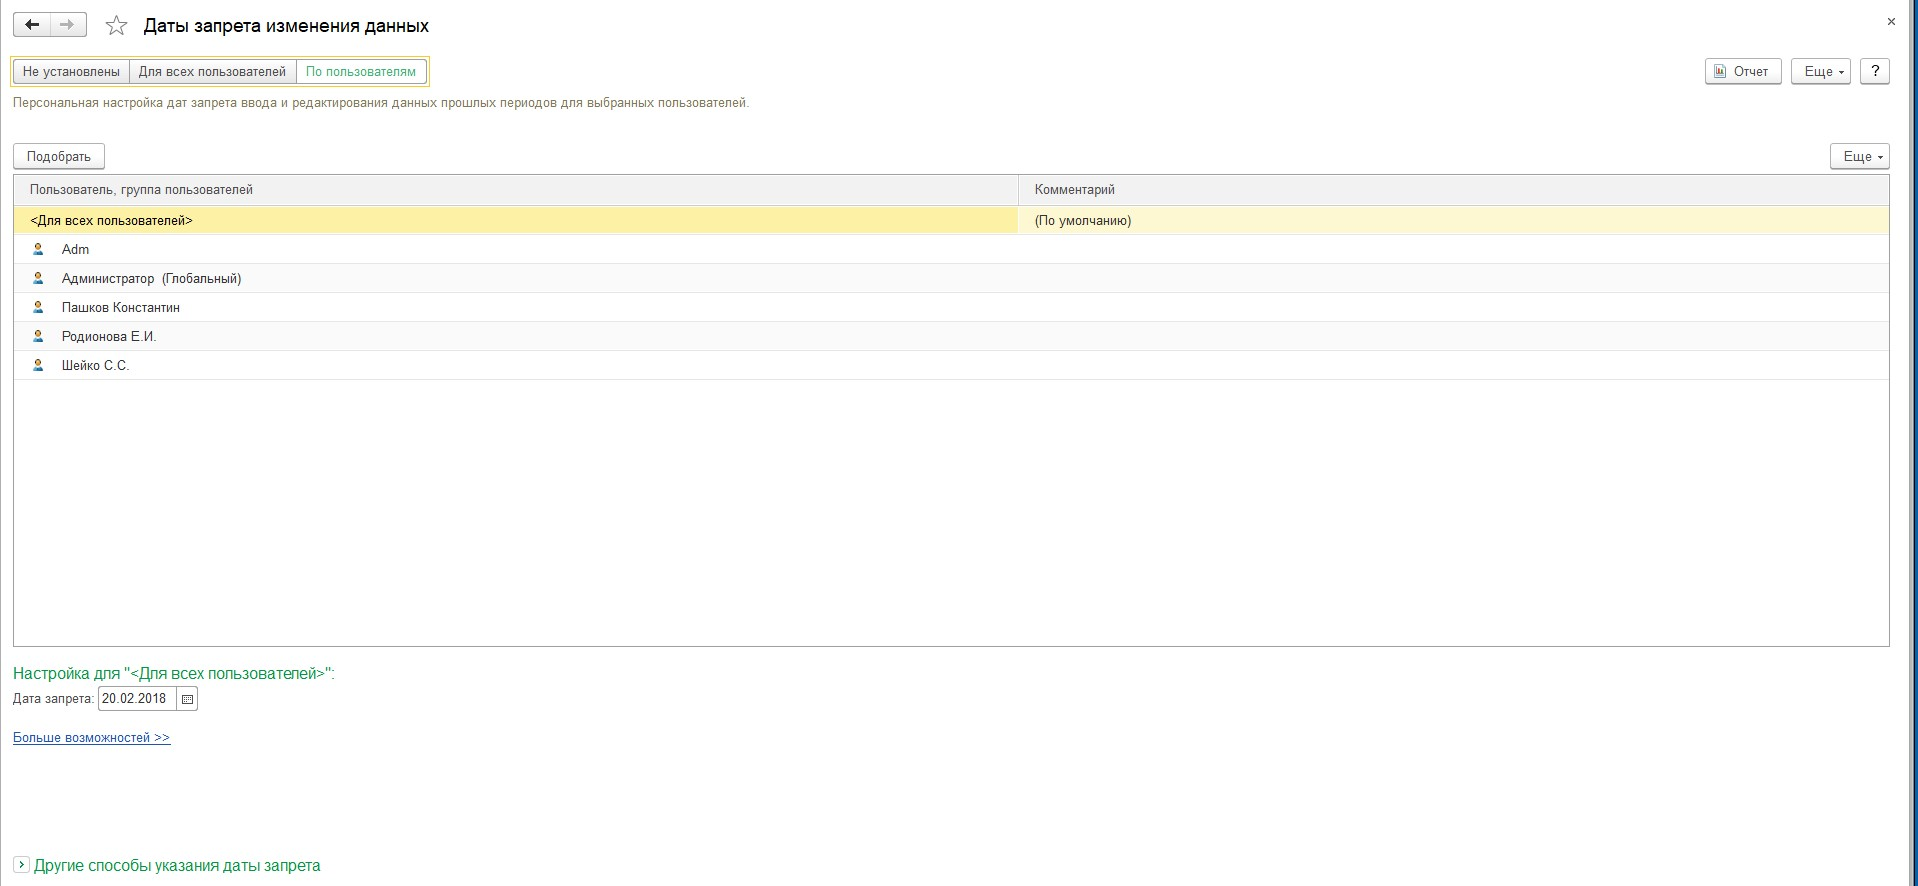
\includegraphics[width=0.85\linewidth]{4.jpg}\label{ris:4.jpg}}
			   \ffigbox{\caption{Эквайринг!}}%
			   {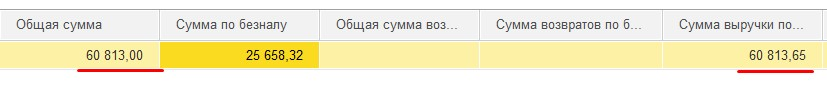
\includegraphics[width=0.85\linewidth]{5.jpg}\label{ris:5.jpg}}         
		   \end{floatrow}
    \end{figure}
	\par
	
		\item На (Рис.~\ref{ris:4.jpg}) цифрами 1. 2. 3. 4 обозначены поля, суммы из которых подлежат вводу в показанную форму  (Рис.~\ref{ris:3.jpg}). При получении  контрольной ленты сверки итогов по эквайрингу (Рис.~\ref{ris:5.jpg})  убедиться, что на контрольной ленте  присутствует надпись «Итоги совпали» (поз. 1) (Рис.~\ref{ris:5.jpg}). После этого найти на ленте итоговую сумму (поз. 2) (Рис.~\ref{ris:5.jpg}) и занести ее в строку (самую нижнюю) под номером 5 формы ввода сумм (Рис.~\ref{ris:3.jpg}). Нажать <<Готово>>.
		
		
		
\end{itemize}
\newpage